\documentclass[12pt, border=12pt]{standalone}
\usepackage[utf8]{inputenc}
\usepackage[utf8]{vietnam}
\usepackage{amsmath,amsfonts,amssymb}
\usepackage{type1cm}
\usepackage{graphicx}
\usepackage{multirow}
\usepackage{multicol}
\usepackage{array}
\usepackage{comment}
\usepackage[unicode]{hyperref}
\usepackage{tikz}
\usepackage{color}
\usepackage[american,cuteinductors,smartlabels]{circuitikz}
\usetikzlibrary{arrows}
\usepackage{tikz}
\usetikzlibrary{calc,patterns,angles,quotes}
\usetikzlibrary{arrows, decorations.markings, calc, fadings, decorations.pathreplacing, patterns, decorations.pathmorphing, positioning}	
%\tikzstyle{every path}=[line width=1.2pt]

\tikzset{middlearrow/.style={
        decoration={markings,
            mark= at position 0.5 with {\arrow{#1}} ,
        },
        postaction={decorate}
    }
}
\begin{document}
	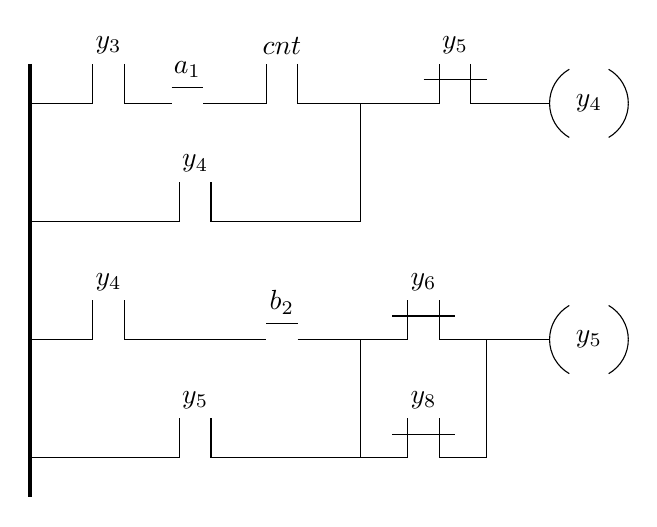
\begin{tikzpicture}[>=triangle 45]
		\draw[ultra thick] (0,-14.5) -- (0,-20);		
		\draw (0,-15) -- (0.8,-15) -- (0.8,-14.5); \draw (1.2,-14.5) -- (1.2,-15) -- (1.8,-15); \draw (1,-14.5) node[above]{$y_{3}$};  \draw (1.8,-14.8) -- (2.2,-14.8); \draw(2,-14.8) node[above]{$a_{1}$}; \draw (2.2,-15) -- (3,-15) -- (3,-14.5); \draw (3.4,-14.5) -- (3.4,-15) -- (4.2,-15); \draw (3.2,-14.5) node[above] {$cnt$};
						
		\draw (4.2,-15) -- (5.2,-15)-- (5.2,-14.5); \draw (5.6,-14.5) -- (5.6,-15) -- (6.6,-15); \draw (5,-14.7) -- (5.8, -14.7); \draw (5.4,-14.5) node[above]{$y_5$};\draw (6.6,-15) arc (180:120:.5);\draw (6.6,-15) arc (180:240:.5); \draw (7.6,-15) arc (0:60:.5);\draw (7.6,-15) arc (0:-60:.5); \draw (7.1,-15) node{$y_4$};
						
		\draw (0,-16.5) -- (1.9,-16.5) -- (1.9,-16); \draw (2.3,-16) -- (2.3,-16.5) -- (4.2,-16.5) -- (4.2,-15); \draw (2.1,-16) node[above]{$y_4$}; 
						
						
		\draw (0,-18) -- (0.8,-18) -- (0.8,-17.5); \draw (1.2,-17.5) -- (1.2,-18) -- (3,-18); \draw (1,-17.5) node[above]{$y_4$}; \draw (3,-17.8) -- (3.4,-17.8); \draw(3.2,-17.8) node[above]{$b_2$}; \draw (3.4,-18) -- (4.2,-18); \draw (4.2,-18) -- (4.8,-18)-- (4.8,-17.5); \draw (5.2,-17.5) -- (5.2,-18) -- (6.6,-18); \draw (4.6,-17.7) -- (5.4, -17.7); \draw (5,-17.5) node[above]{$y_6$}; 
		\draw (6.6,-18) arc (180:120:.5);\draw (6.6,-18) arc (180:240:.5); \draw (7.6,-18) arc (0:60:.5);\draw (7.6,-18) arc (0:-60:.5); \draw (7.1,-18) node{$y_5$}; \draw (0,-19.5) -- (1.9,-19.5) -- (1.9,-19); \draw (2.3,-19) -- (2.3,-19.5) -- (4.2,-19.5) -- (4.2,-18); \draw (2.1,-19) node[above]{$y_5$};
								
		\draw (4.2,-19.5) -- (4.8,-19.5)-- (4.8,-19); \draw (5.2,-19) -- (5.2,-19.5) -- (5.8,-19.5) -- (5.8,-18); \draw (4.6,-19.2) -- (5.4, -19.2); \draw (5,-19) node[above]{$y_8$};		
	\end{tikzpicture}
\end{document}